\section{卷积:常量内存和缓存简介}
在接下来的几章中,我们将讨论一组重要的并行计算模式。 这些模式是许多并行应用中出现的各种并行算法的基础。 
我们将从卷积开始,它是一种流行的数组运算,在信号处理、数字记录、图像处理、视频处理和计算机视觉中以多种形式使用。 
在这些应用领域中,卷积通常作为滤波器来执行,将信号和像素转换为更理想的值。 
我们的图像模糊内核就是这样一个滤波器,它可以平滑信号值,以便人们可以看到大图趋势。 
又例如,高斯滤波器是卷积滤波器,可用于锐化图像中对象的边界和边缘。

卷积通常执行大量算术运算来生成每个输出元素。 对于高清图像和视频等输出元素(像素)较多的大型数据集,计算量可能会很大。 
一方面,卷积的每个输出数据元素可以彼此独立地计算,这是并行计算的理想特性。 
另一方面,在处理具有一定挑战性的边界条件的不同输出数据元素时存在大量输入数据共享。 
这使得卷积成为复杂的平铺方法和输入数据分级方法的重要用例,这也是本章的重点。

\subsection{背景}
卷积是一种数组运算,其中每个输出数据元素是相应输入元素和以其为中心的输入元素集合的加权和。 
加权和计算中使用的权重由滤波器数组定义,通常称为卷积核。 
由于 CUDA 内核函数和卷积内核之间存在不幸的名称冲突,因此我们将这些滤波器数组称为卷积滤波器以避免混淆。

可以对不同维度的输入数据执行卷积:一维 (1D)(例如音频)、二维 (2D)(例如照片)、三维 (3D)(例如视频)等 。 
在音频数字信号处理中,输入一维阵列元素是随时间变化的采样信号量。 也就是说,输入数据元素 $x_i$ 是音频信号音量的第i个样本。 
一维数据上的卷积(称为一维卷积)在数学上定义为一个函数,
该函数采用 n 个元素的输入数据数组 $[x_0 , x_1 , \ldots , x_{n-1} ]$ 
和 2r + 1 个元素的滤波器数组 $[f_0 , f_1 , \ldots , f_{2r} ]$ 并返回输出数据数组 y:

$$
y_i = \sum^r_{j=-r} f_{i+j}\times x_i
$$

由于滤波器的大小为奇数($2r + 1$),因此加权和计算围绕正在计算的元素是对称的。
也就是说,加权和涉及正在计算的位置每一侧的 r 个输入元素, 这就是为什么 r 被称为滤波器半径的原因。

\begin{figure}[H]
	\centering
	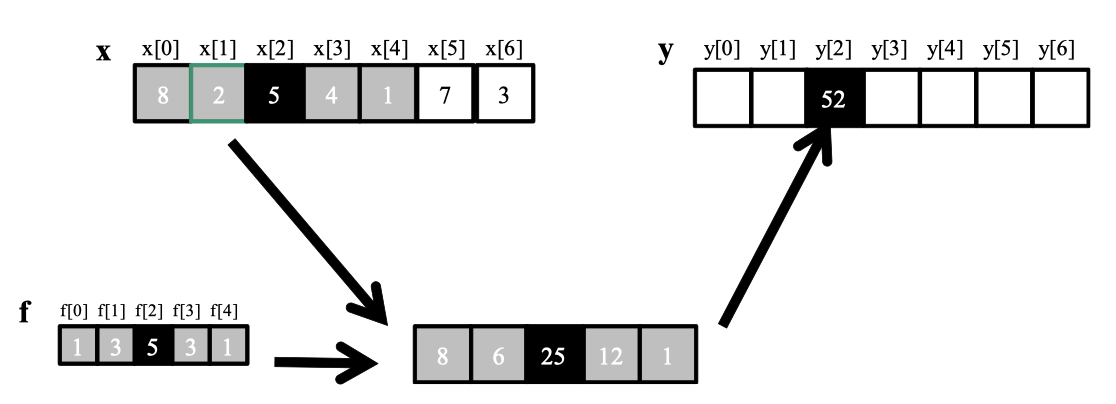
\includegraphics[width=0.9\textwidth]{figs/F7.1.png}
	\caption{\textit{元素内部的一维卷积示例。}}
\end{figure}

图 7.1 显示了一个一维卷积示例,其中将五元素($r = 2$)卷积滤波器 $f$ 应用于七元素输入数组 $x$。 
我们将遵循 C 语言约定,其中 $x$ 和 $y$ 元素的索引从 0 到 6,$f$ 元素的索引从 0 到 4。
由于过滤器半径为 2,因此每个输出元素计算为相应输入元素的加权和 ,左侧有两个元素,右侧有两个元素。

例如,$y[2]$ 的值被生成为 $x[0]$(即 $x[2 - 2]$)到 $x[4]$(即 $x[2 + 2]$)的加权和。 
在此示例中,我们任意假设 $x$ 元素的值为 $[8, 2, 5, 4, 1, 7, 3]$。 
$f$ 元素定义权重,在此示例中其值为 $1, 3, 5, 3, 1$。 
每个 $f$ 元素先与相应的 $x$ 元素值相乘,然后再将乘积相加。 如图7.1所示,$y[2]$ 的计算如下:
$$
\begin{aligned}
y[2] & =f[0]^{*} x[0]+f[1]^{*} x[1]+f[2]^{*} x[2]+f[3]^{*} x[3]+f[4]^{*} x[4] \\
& =1^{*} 8+3^{*} 2+5^{*} 5+3^{*} 4+1^{*} 1 \\
& =52
\end{aligned}
$$

\begin{figure}[H]
	\centering
	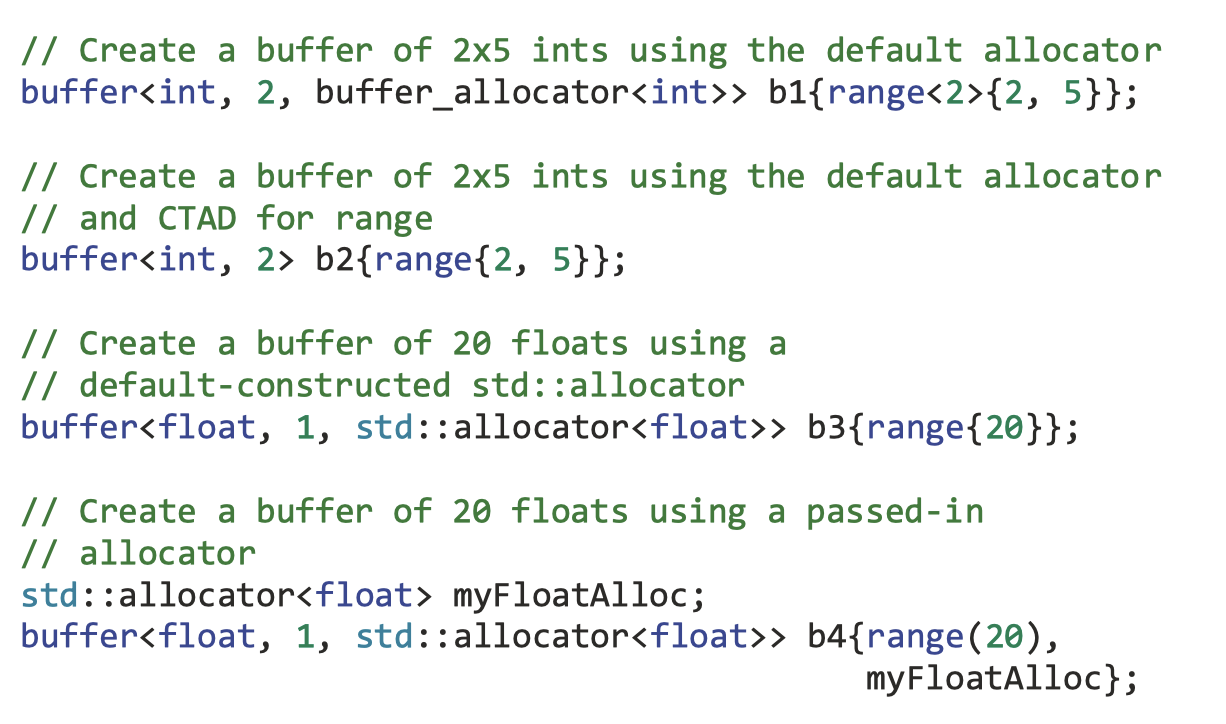
\includegraphics[width=0.9\textwidth]{figs/F7.2.png}
	\caption{\textit{一维卷积,y[3]的计算。}}
\end{figure}

在图 7.1 中,$y[i]$ 的计算可以看作是从 $x[I - 2]$ 开始的 $x$ 子数组与 $f$ 数组之间的内积。 
图 7.2 显示了 $y[3]$ 的计算。 该计算与图 7.1 的计算相比移动了一个 x 元素。 
也就是说,$y[3]$ 的值是 $x[1]$(即 $x[3 - 2]$)到 $x[5]$(即 x[3 + 2])的加权和。 
我们可以认为x[3]的计算如下内积:
$$
\begin{aligned}
y[3] & =f[0]^{*} x[1]+f[1]^{*} x[2]+f[2]^{*} x[3]+f[3]^{*} x[4]+f[4]^{*} x[5] y[3] \\
& =f[0]^{*} x[1]+f[1]^{*} x[2]+f[2]^{*} x[3]+f[3]^{*} x[4]+f[4]^{*} x[5] \\
& =1^{*} 2+3^{*} 5+5^{*} 4+3^{*} 1+1^{*} 7 \\
& =47
\end{aligned}
$$

\begin{figure}[H]
	\centering
	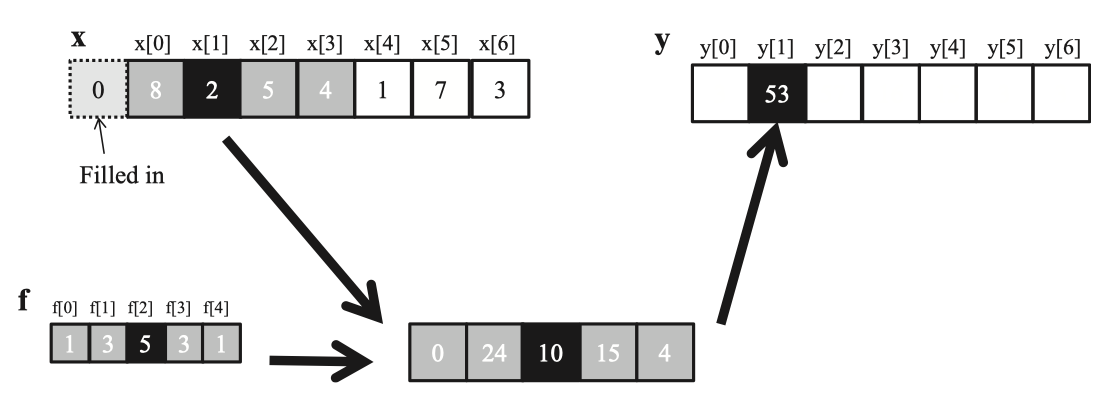
\includegraphics[width=0.9\textwidth]{figs/F7.3.png}
	\caption{\textit{一维卷积边界条件。}}
\end{figure}

由于卷积是根据相邻元素定义的,因此在计算靠近数组末端的输出元素时自然会出现边界条件。 
如图7.3所示,当我们计算y[1]时,x[1]左边只有一个x元素。 也就是说,根据我们对卷积的定义,没有足够的 x 元素来计算 y[1]。 
处理此类边界条件的典型方法是为这些缺失的 x 元素分配默认值。 
对于大多数应用程序,默认值为 0,这就是我们在图 7.3 中使用的值。 
例如,在音频信号处理中,我们可以假设录音开始之前和结束之后信号音量为0。 此时,y[1]的计算如下:
$$
\begin{aligned}
y[1] & =f[0]^{*} 0+f[1]^{*} x[0]+f[2]^{*} x[1]+f[3]^{*} x[2]+f[4]^{*} x[3] \\
& =1^{*} 0+3^{*} 8+5^{*} 2+3^{*} 5+1^{*} 4 \\
& =53
\end{aligned}
$$

本次计算中不存在的 x 元素如图 7.3 中的虚线框所示。 
应该清楚的是,y[0] 的计算将涉及两个缺失的 x 元素,在本例中,这两个元素都将被假定为 0。 
我们将 y[0] 的计算作为练习。 这些缺失的元素在文献中通常被称为幻影单元。 
由于在并行计算中使用平铺,还存在其他类型的幻影单元。 这些幻影单元可以对平铺的有效性和/或效率产生重大影响。 
我们很快就会回到这一点。

此外,并非所有应用程序都假设幻影单元包含 0。
例如,某些应用程序可能假设幻影单元包含与边缘上最接近的有效数据元素相同的值。

对于图像处理和计算机视觉,输入数据通常表示为 2D 数组,其中像素位于 $x-y$ 空间中。 
因此,图像卷积是 2D 卷积,如图 7.4 所示。 在 2D 卷积中,滤波器 f 也是一个 2D 数组。 
它的 x 和 y 维度确定了要包含在加权和计算中的邻居的范围。 
如果我们假设滤波器的x维度维度为($2r_x + 1$),y维度维度为($2r_y + 1$),则每个P元素的计算可以表达如下:
$$
P_{y, x}=\sum_{j=-r_{y}}^{r_{y}} \sum_{k=-r_{x}}^{r_{x}} f_{y+j, x+k} \quad \times N_{y, x}
$$

\begin{figure}[H]
	\centering
	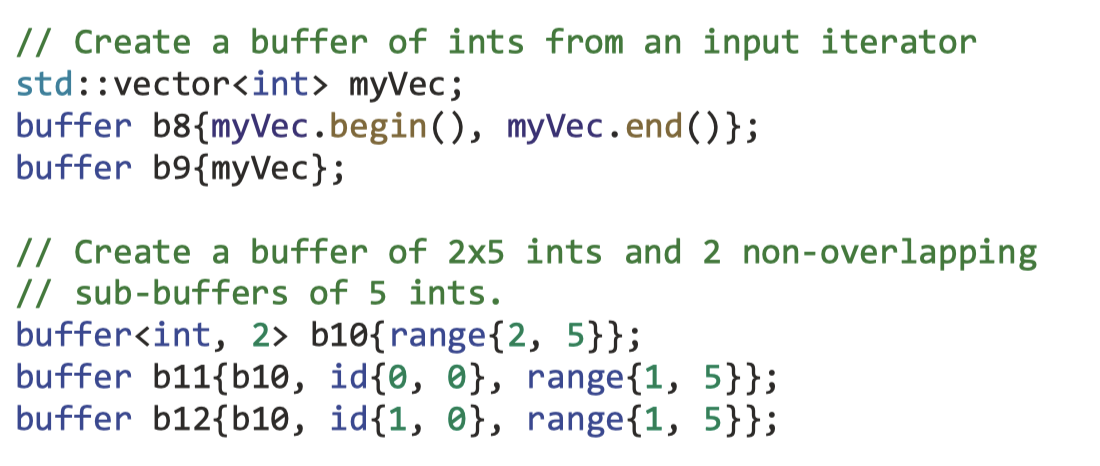
\includegraphics[width=0.9\textwidth]{figs/F7.4.png}
	\caption{\textit{2D 卷积示例。}}
\end{figure}

在图 7.4 中,为了简单起见,我们使用 $5 \times 5$ 滤波器; 即,$r_y = 2$ 且 $r_x = 2$。
一般来说,滤波器不必是但通常是方阵。 为了生成输出元素,我们采用中心位于输入数组 N 中相应位置的子数组。
然后,我们在滤波器数组的元素和图像数组的元素之间执行成对乘法。 
对于我们的示例,结果显示为图 7.4 中 N 和 P 下方的 $5 \times 5$ 乘积数组。 输出元素的值是乘积数组所有元素的总和。

图 7.4 中的示例显示了 P2,2 的计算。 为简洁起见,在寻址 C 数组时,我们将使用 Ny,x 来表示 N[y][x]。 
由于 N 和 P 很可能是动态分配的数组,因此我们将在实际代码示例中使用线性化索引。 计算如下:

\begin{figure}[H]
	\centering
	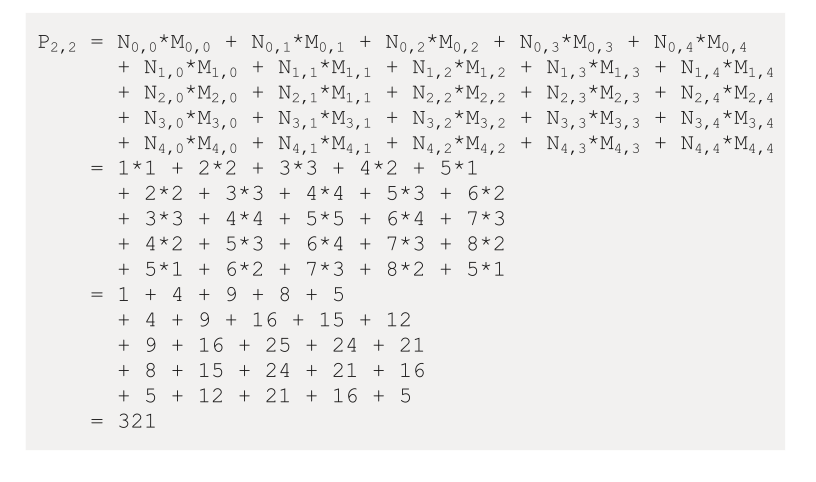
\includegraphics[width=0.9\textwidth]{figs/F7-a1.png}
\end{figure}

\begin{figure}[H]
	\centering
	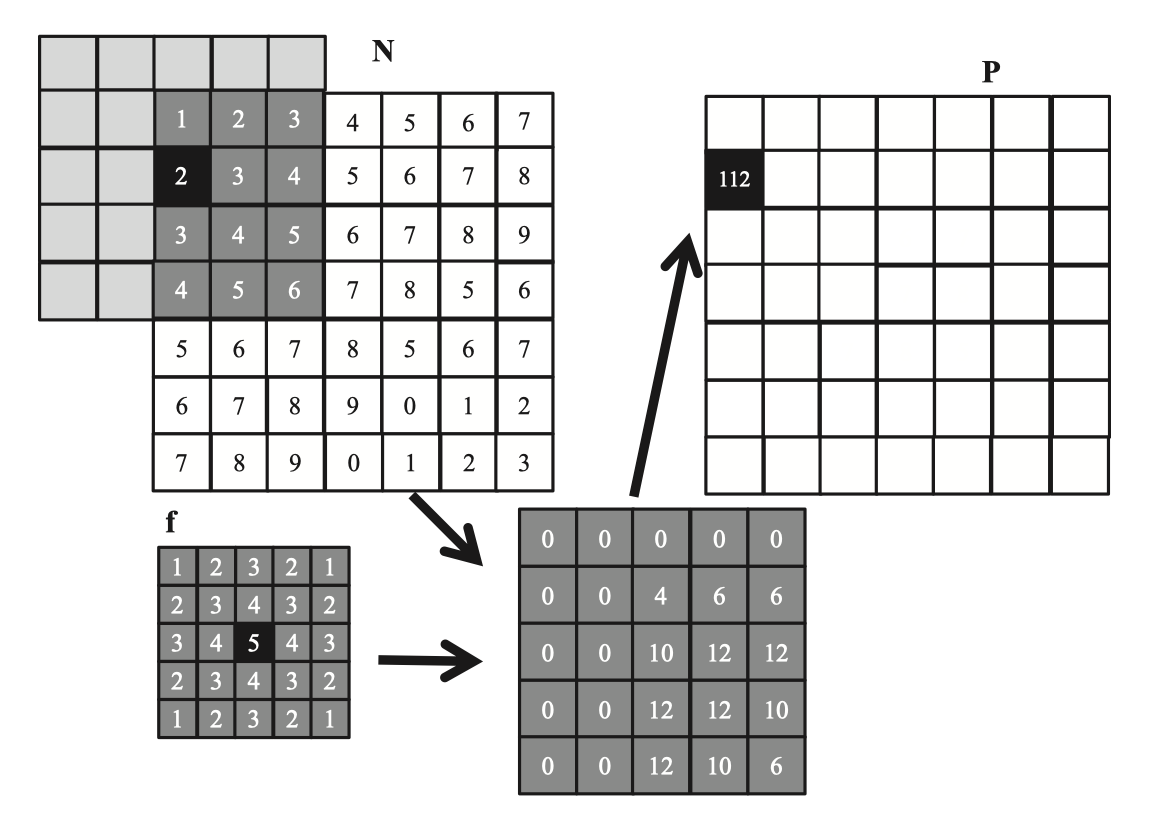
\includegraphics[width=0.9\textwidth]{figs/F7.5.png}
	\caption{\textit{二维卷积边界条件。}}
\end{figure}

与一维卷积一样,二维卷积也必须处理边界条件。 
对于 x 和 y 维度上的边界,存在更复杂的边界条件:输出元素的计算可能涉及沿水平边界、垂直边界或两者的边界条件。 
图 7.5 说明了涉及两个边界的 $P$ 元素的计算。 从图 7.5 中,$P_{1,0}$ 的计算涉及 $N$ 子数组中的两列缺失和一行缺失。
与一维卷积一样,不同的应用程序对这些缺失的 $N$ 个元素假设不同的默认值。 
在我们的示例中,我们假设默认值为 0。这些边界条件也会影响平铺的效率。 我们很快就会回到这一点。

\subsection{并行卷积:基础算法}
事实上,所有输出元素的计算都可以在卷积中并行完成,这使得卷积成为并行计算的理想用例。 
根据我们在矩阵乘法方面的经验,我们可以快速编写一个简单的并行卷积核。 
我们将展示 2D 卷积的代码示例,并鼓励读者将这些代码示例改编为 1D 和 3D 作为练习。 
另外,为了简单起见,我们将假设方形滤波器。

第一步是定义内核的主要输入参数。 我们假设 2D 卷积核接收五个参数:指向输入数组 N 的指针; 指向过滤器的指针 F; 
指向输出数组 P 的指针; 方形滤波器的半径,r; 输入和输出数组的宽度,width; 以及输入和输出数组的高度 height。 
因此我们有以下设置:

\begin{figure}[H]
	\centering
	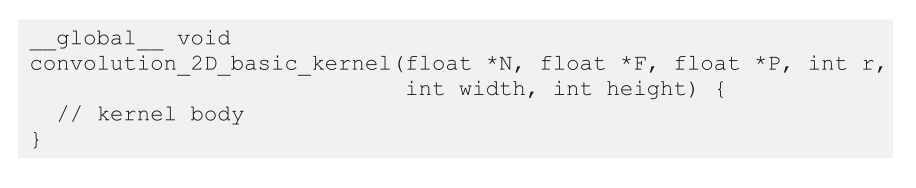
\includegraphics[width=0.9\textwidth]{figs/F7-a2.png}
\end{figure}

第二步是确定并实现线程到输出元素的映射。 由于输出数组是二维的,一种简单而好的方法是将线程组织成二维网格,
并让网格中的每个线程计算一个输出元素。 每个块最多可以有 1024 个线程,最多可以计算 1024 个输出元素。 
图 7.6 显示了一个玩具示例,其中输入和输出为 $16 \times 16$ 个图像。 
我们假设在此玩具示例中,每个线程块都组织为 $4 \times 4$ 线程数组:x 维度有四个线程,y 维度有四个线程。 
本例中的网格被组织为 $4 \times 4$ 块数组。 
将线程分配给输出元素(本例中为输出像素)很简单:分配每个线程来计算一个输出像素,其 x 和 y 索引与线程的 x 和 y 索引相同。

\begin{figure}[H]
	\centering
	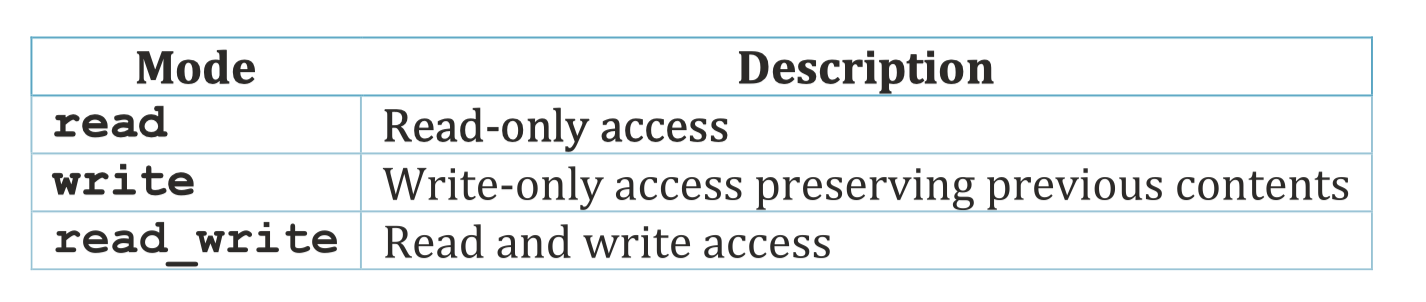
\includegraphics[width=0.9\textwidth]{figs/F7.6.png}
	\caption{\textit{2D 卷积的并行化和线程组织。}}
\end{figure}

\begin{figure}[H]
	\centering
	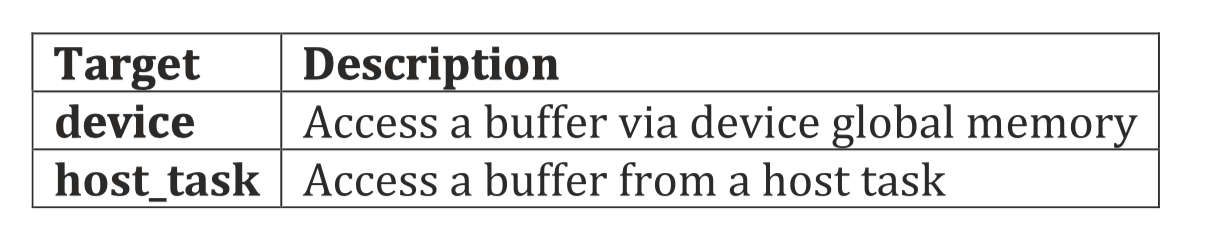
\includegraphics[width=0.9\textwidth]{figs/F7.7.png}
	\caption{\textit{具有边界条件处理的 2D 卷积核。}}
\end{figure}

读者应该认识到图 7.6 中的并行化安排与第 3 章“多维网格和数据”中的 ColorToGrayScaleConversion 示例相同。 
因此,我们可以使用图 7.7 中内核的第 02 行和第 03 行中的语句,根据每个线程的块索引、块维度和线程索引来计算输出元素索引。 
例如,$block_{1,1}$ 的 $thread_{1,1}$ 映射到输出元素 P[1 $\times$ 4+1][1 $\times$ 4+1]=P[5][5],
在图 7.6 中标记为绿色方块。

一旦确定了每个线程的输出元素索引,我们就可以识别计算输出元素所需的输入 N 个元素。 
如图 7.6 所示,$block_{1, 1}$ 的 $thread_{1, 1}$ 计算 P[5][5](绿色方块)时
将使用 x 索引范围从 outCol - r=3 到 outCol + r 的输入元素 =7,其 y 索引范围从 outRow - r = 3 到 outRow + r=7。 
对于所有线程,outCol - r 和 outRow - r 定义 P[outRow][outCol] 所需的
输入元素块(浅阴影区域)的左上角(重阴影正方形)。 
因此,我们可以使用双重嵌套循环来迭代所有这些索引值并执行此计算(图 7.7 的第 05-13 行)。

寄存器变量 Pvalue 将累积所有中间结果以节省 DRAM 带宽。 
内部 for 循环中的 if 语句测试所使用的任何输入 N 元素是否是 N 数组左侧、右侧、顶部或底部的幻影单元。 
由于我们假设 0 值将用于幻影单元,因此我们可以简单地跳过幻影单元元素及其相应过滤元素的乘法和累加。 
循环结束后,我们将 Pvalue 释放到输出 P 元素中(第 14 行)。

我们对图 7.7 中的内核进行了两个观察。 首先,会出现控制流发散。 
计算 P 数组四个边缘附近的输出元素的线程将需要处理幻影单元。 正如我们在 7.1 节中所示,每个线程都会遇到不同数量的幻影单元。 
因此,它们在 if 语句(第 09 行)中的决定都有些不同。 
计算 P[0][0] 的线程大多数时候会跳过乘法累加语句,而计算 P[0][1] 的线程会跳过较少的次数,依此类推。 
控制发散的成本将取决于输入数组的宽度和高度的值以及滤波器的半径。 
对于大型输入数组和小型滤波器,控制发散仅发生在计算一小部分输出元素时,这将使控制发散的影响保持较小。 
由于卷积通常应用于大图像,因此我们预计控制散度的影响范围从适度到微不足道。

更严重的问题是内存带宽。 浮点算术计算与全局内存访问的比率仅为约0.25 OP/B(第10行加载的每8字节2次操作)。 
正如我们在矩阵乘法示例中看到的,这个简单的内核预计只能以峰值性能的一小部分运行。 
我们将在接下来的两节中讨论减少全局内存访问次数的两种关键技术。

\subsection{常量内存与缓存}
滤波器阵列 F 在卷积中的使用方式存在三个有趣的属性。 首先,F的尺寸通常很小; 大多数卷积滤波器的半径为 7 或更小。 
即使在 3D 卷积中,滤波器通常也仅包含小于或等于 $7^3 = 343$ 个元素。 其次,F的内容在卷积核的执行过程中不会改变。 
第三,所有线程都访问过滤器元素。 
更好的是,所有线程都以相同的顺序访问 F 元素,从 F[0][0] 开始,通过图 7.7 中的双重嵌套 for 循环的迭代一次移动一个元素。 
这三个属性使过滤器成为常量内存和缓存的绝佳候选者(图 7.8)。

\begin{figure}[H]
	\centering
	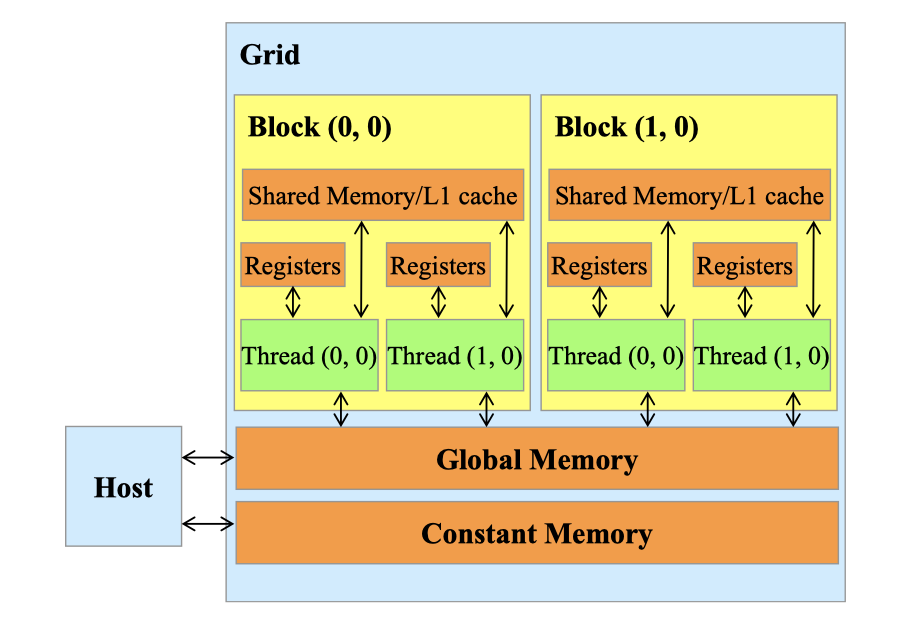
\includegraphics[width=0.9\textwidth]{figs/F7.8.png}
	\caption{\textit{CUDA 内存模型回顾。}}
\end{figure}

正如我们在第 5 章“内存架构和数据局部性”(表 5.1)中讨论的那样,CUDA C 允许程序员声明驻留在常量内存中的变量。 
与全局内存变量一样,常量内存变量对所有线程块都是可见的。 主要区别在于常量内存变量的值在内核执行期间不能被线程修改。 
此外,常量内存的大小非常小,目前为 64 KB。

要使用常量内存,主机代码需要以与全局内存变量不同的方式分配和复制常量内存变量。 
我们假设过滤器的半径在编译时常量 FILTER\_RADIUS 中指定。 
要在常量内存中声明 F 数组,主机代码将其声明为全局变量,如下所示:

\begin{figure}[H]
	\centering
	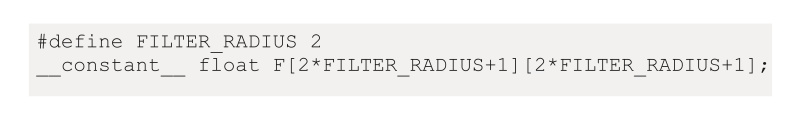
\includegraphics[width=0.9\textwidth]{figs/F7-a3.png}
\end{figure}

请注意,这是一个全局变量声明,应该位于源文件中的任何函数之外。 
关键字 \_\_constant\_\_ (每边两个下划线)告诉编译器数组 F 应放入设备常量内存中。

假设主机代码已经在主机存储器中的过滤器 F\_h 数组中分配并初始化了掩码,其中包含 (2 $\times$ FILTER\_RADIUS+1)2 个元素。 
F\_h 的内容可以从主机存储器传输到设备常量存储器中的 F,如下所示:

\begin{figure}[H]
	\centering
	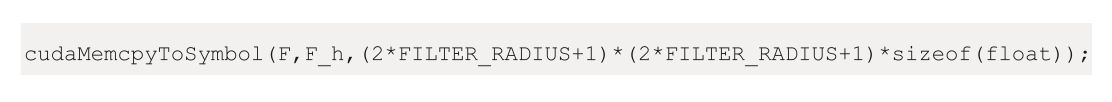
\includegraphics[width=0.9\textwidth]{figs/F7-a4.png}
\end{figure}

请注意,这是一个特殊的内存复制函数,它通知 CUDA 运行时复制到常量内存中的数据在内核执行期间不会更改。 
一般来说,cudaMemcpyToSymble()函数的使用如下:

\begin{figure}[H]
	\centering
	
\includegraphics[width=0.9\textwidth]{figs/F7-a5.png}
\end{figure}

其中 dest 是指向常量内存中目标位置的指针,src 是指向主机内存中源数据的指针,size 是要复制的字节数。
\footnote{该函数还可以采用两个参数,即 offset 和 kind,但它们很少使用并且经常被省略。 
读者可参阅《CUDA C 编程指南》以了解这些参数的详细信息。}

\begin{figure}[H]
	\centering
	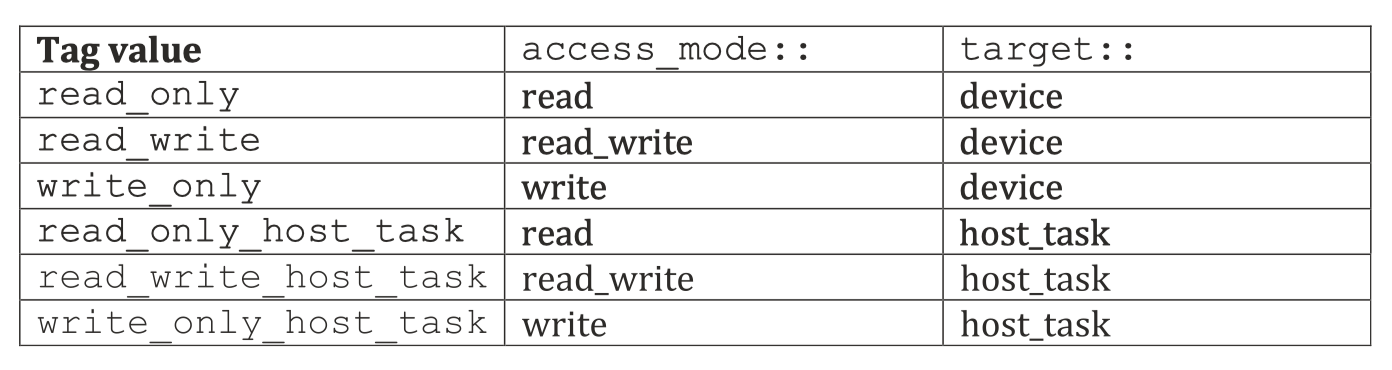
\includegraphics[width=0.9\textwidth]{figs/F7.9.png}
	\caption{\textit{使用 F 常量内存的 2D 卷积核。}}
\end{figure}

内核函数将常量内存变量作为全局变量访问。 因此它们的指针不需要作为参数传递给内核。 
我们可以修改内核以使用常量内存,如图 7.9 所示。 请注意,内核看起来与图 7.7 中的内核几乎相同。 
唯一的区别是 F 不再通过作为参数传入的指针来访问。 现在它作为全局变量进行访问。 
请记住,全局变量的所有 C 语言作用域规则都适用于此处。 
如果主机代码和内核代码在不同的文件中,则内核代码文件必须包含相关的外部声明信息,以保证F的声明对内核可见。

与全局内存变量一样,常量内存变量也位于 DRAM 中。 
然而,由于 CUDA 运行时知道常量内存变量在内核执行期间不会被修改,因此它指示硬件在内核执行期间积极缓存常量内存变量。 
要了解常量内存使用的好处,我们需要首先了解有关现代处理器内存和缓存层次结构的更多信息。

正如我们在第 6 章“性能注意事项”中讨论的那样,DRAM 的长延迟和有限带宽构成了几乎所有现代处理器的瓶颈。 
为了减轻内存瓶颈的影响,现代处理器通常采用片上高速缓冲存储器或高速缓存,
以减少需要从主内存 (DRAM) 访问的变量数量,如图 7.10 所示。

\begin{figure}[H]
	\centering
	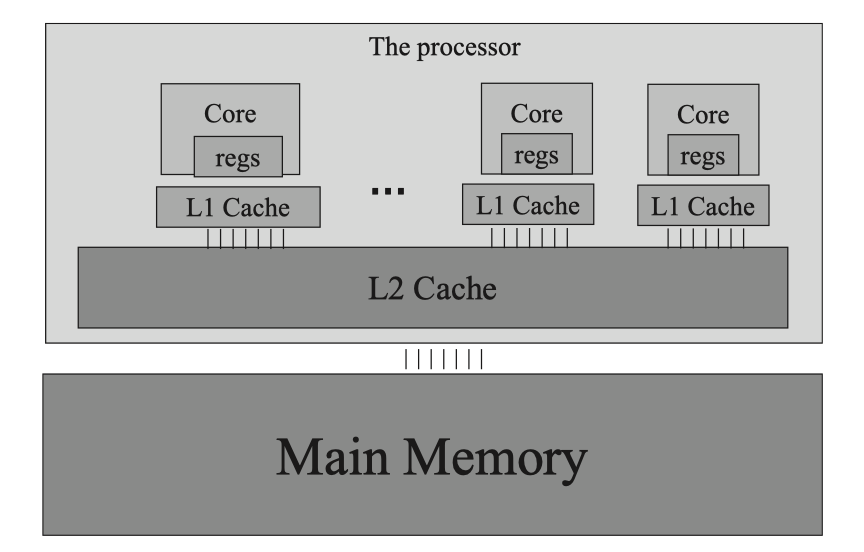
\includegraphics[width=0.9\textwidth]{figs/F7.10.png}
	\caption{\textit{现代处理器缓存层次结构的简化视图。}}
\end{figure}

与 CUDA 共享内存或一般的暂存器内存不同,缓存对程序是“透明的”。 
也就是说,要使用 CUDA 共享内存来保存全局变量的值,
程序需要将变量声明为 \_\_shared\_\_ 并显式地将全局内存变量的值复制到共享内存变量中。 
另一方面,在使用缓存时,程序只是访问原始的全局内存变量。 处理器硬件会自动将最近或经常使用的变量保留在缓存中,
并记住它们原来的全局内存地址。 当稍后使用保留的变量之一时,硬件将从它们的地址检测到该变量的副本在缓存中可用。 
然后将从缓存中提供变量的值,从而无需访问 DRAM。

在存储器的大小和存储器的速度之间存在权衡。 因此,现代处理器通常采用多级缓存。 
这些高速缓存级别的编号约定反映了到处理器的距离。 最低级别 L1 或级别 1 是直接连接到处理器内核的高速缓存,
如图 7.10 所示。 它的运行速度在延迟和带宽方面都接近处理器的运行速度。 
然而,L1 缓存容量较小,通常在 16 到 64 KB 之间。 
L2 缓存更大,范围为几百 KB 到少量 MB,但可能需要数十个周期才能访问。 
它们通常在 CUDA 设备中的多个处理器核心或流式多处理器 (SM) 之间共享,因此访问带宽在 SM 之间共享。 
在当今的一些高端处理器中,甚至有大小可达数百兆字节的三级缓存。

常量内存变量在大规模并行处理器中设计和使用内存时发挥着有趣的作用。 
由于这些常量内存变量在内核执行期间不会被修改,因此在将它们缓存在 SM 中时不需要支持线程写入。 
支持对通用缓存的高吞吐量写入需要复杂的硬件逻辑,并且在芯片面积和功耗方面成本高昂。 
在不需要支持写入的情况下,可以在芯片面积和功耗方面以高效的方式设计用于常量存储器变量的专用高速缓存。 
此外,由于常量内存非常小(64 KB),因此小型专用缓存可以非常有效地捕获每个内核大量使用的常量内存变量。 
这种专用缓存在现代 GPU 中称为常量缓存。 
因此,当一个 warp 中的所有线程访问相同的常量内存变量时,如图 7.9 中的 F 的情况,其中访问 F 的索引独立于线程索引,
常量缓存可以提供大量的常量内存变量。 带宽以满足这些线程的数据需求。 
此外,由于 F 的大小通常很小,因此我们可以假设所有 F 元素实际上总是从常量高速缓存访问。 
因此,我们可以简单地假设没有 DRAM 带宽用于访问 F 元素。 
通过使用常量内存和缓存,我们有效地将浮点运算与内存访问的比率增加了一倍,
达到约 0.5 OP/B(第 10 行加载的每 4 个字节执行 2 次操作)。

事实证明,对输入 N 数组元素的访问也可以从缓存中受益。 我们将在 7.5 节中回到这一点。

\subsection{带环单元的平铺卷积}
我们可以通过平铺卷积算法解决卷积的内存带宽瓶颈。 
回想一下,在平铺算法中,线程协作将输入元素加载到片上存储器中,以便后续使用这些元素。 
我们将首先建立输入和输出图块的定义,因为这些定义对于理解算法的设计非常重要。 
我们将每个块处理的输出元素的集合称为输出图块。 
回想一下,图 7.6 显示了 $16 \times 16$ 2D 卷积的玩具示例,该卷积使用 16 个块,每个块有 16 个线程。 
在该示例中,有 16 个输出图块。 请记住,我们每个块使用 16 个线程来保持示例较小。 
实际上,每个块应该至少有 32 个线程或 1 个线程束,通常更多,以实现良好的占用和数据重用。 
从现在开始,我们假设 F 元素位于常量存储器中。

\begin{figure}[H]
	\centering
	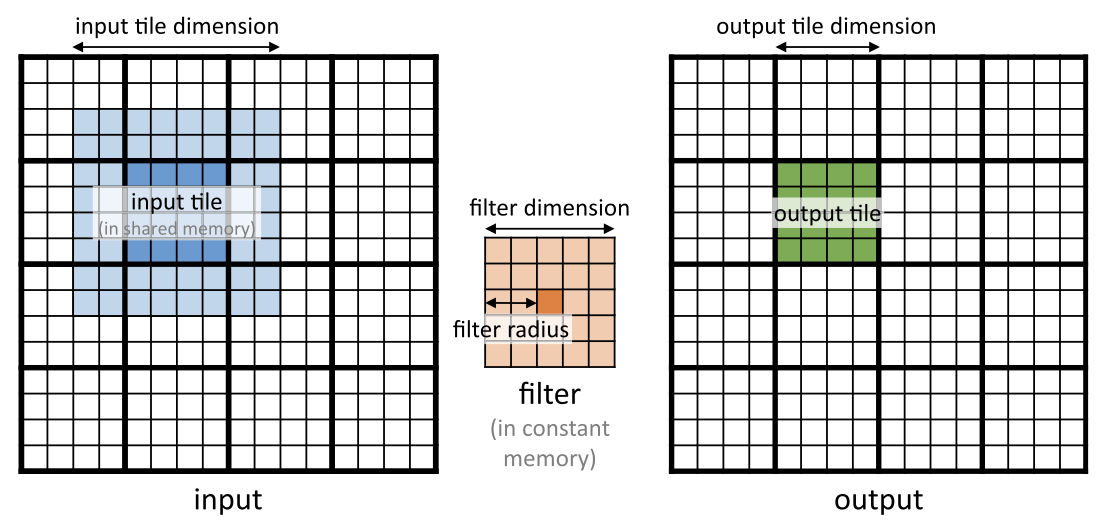
\includegraphics[width=0.9\textwidth]{figs/F7.11.png}
	\caption{\textit{2D 卷积中的输入图块与输出图块。}}
\end{figure}

我们将输入图块定义为计算输出图块中的 P 个元素所需的输入 N 个元素的集合。 
图 7.11 显示了与输出图块(右侧的阴影块)相对应的输入图块(左侧的阴影块)。 
请注意,输入图块的尺寸需要在每个方向上扩展滤波器的半径(本例中为 2),
以确保它包括计算输出图块边缘的 P 元素所需的所有光环输入元素。 
此扩展可以使输入图块明显大于输出图块。 
在此玩具示例中,每个输出图块由 $4^2 = 16$ 个 P 元素组成,而每个输入图块由 $(4 + 4)^2 = 8^2 = 64$ 个元素组成。 
在这种情况下,输入图块比输出图块大 $4\times$。 然而,如此大的比率是因为我们假设输出图块尺寸很小,以便于玩具示例中的可视化。 
实际上,输出图块尺寸会大得多,并且输入图块尺寸和输出图块尺寸之间的比率将接近1.0。 
例如,如果输出大小为 $16 \times 16 = 256$,使用相同的 $5 \times 5$ 滤波器,则输入图块大小将为 $(16 + 4)^2 = 400$。
输入图块大小与输出大小之间的比率约 1.6。 
尽管这个比率远小于 4,但它表明即使对于实际的输出图块尺寸,输入图块尺寸仍然可以明显大于输出图块。

在本节中,我们介绍一类分块卷积算法,其中块中的所有线程首先协作将输入分块加载到共享内存中,
然后通过访问共享内存中的输入元素来计算输出分块的元素。 
这对读者来说应该很熟悉; 该策略类似于第 5 章“内存架构和数据局部性”中讨论的平铺矩阵乘法算法。 
主要区别在于,第 5 章“内存架构和数据局部性”中的分块矩阵乘法算法假设输入分块与输出分块具有相同的维度,
而卷积输入分块大于输出分块。 输入图块大小和输出图块大小之间的差异使图块卷积核的设计变得复杂。

有两个简单的线程组织用于解决输入图块大小和输出图块大小之间的差异。 
第一个启动线程块,其尺寸与输入图块的尺寸匹配。 这简化了输入图块的加载,因为每个线程只需要加载一个输入元素。 
然而,由于块维度大于输出图块的维度,因此在计算输出元素时需要禁用一些线程,这会降低执行资源的利用效率。 
第二种方法启动尺寸与输出图块匹配的块。 
一方面,第二种策略使输入图块加载更加复杂,因为线程需要迭代以确保加载所有输入图块元素。 
另一方面,它简化了输出元素的计算,因为块的维度与输出图块相同,并且在输出元素的计算期间不需要禁用任何线程。 
我们将介绍基于第一个线程组织的内核设计,并将第二个组织作为练习。

\begin{figure}[H]
	\centering
	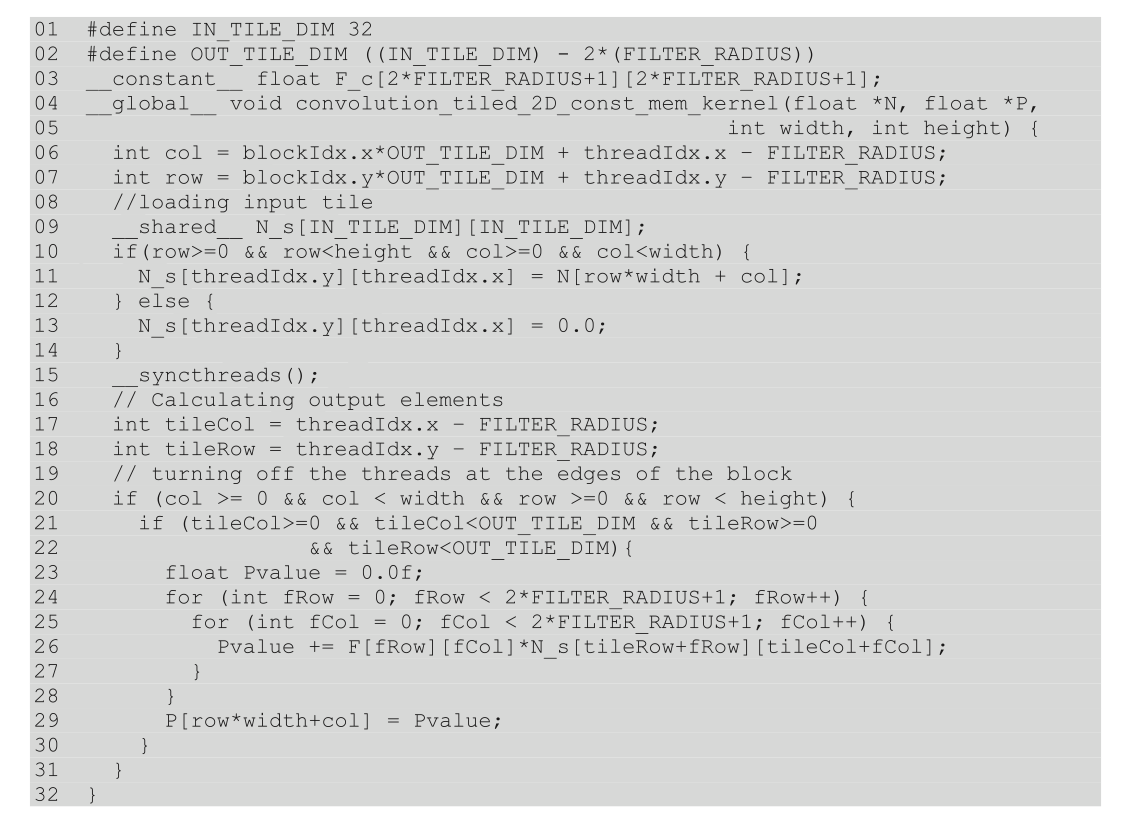
\includegraphics[width=0.9\textwidth]{figs/F7.12.png}
	\caption{\textit{使用 F 的常量内存的平铺 2D 卷积核。}}
\end{figure}

图 7.12 显示了基于第一种线程组织的内核。 
每个线程首先计算它负责加载或计算的输入或输出元素的列索引(col)和行索引(row)(第06-07行)。 
内核分配一个共享内存数组 N\_s,其大小与输入图块相同(第 09 行),并将输入图块加载到共享内存数组(第 10-15 行)。 
每个线程使用第 10 行中的条件来检查它尝试加载的输入图块元素是否为幻影单元。 
如果是,则该线程不执行内存加载。 相反,它会将零放入共享内存中。 
所有线程都执行屏障同步(第 15 行),以确保在允许任何线程继续计算输出元素之前整个输入图块已在共享内存中就位。

现在所有输入图块元素都在 N\_ds 数组中,每个线程可以使用 N\_ds 元素计算其输出 P 元素值。 
请记住,输出图块小于输入图块,并且块与输入图块大小相同,因此仅每个块中的线程子集将用于计算输出图块元素。 
我们可以通过多种方式选择用于此计算的线程。 我们使用一种停用 FILTER\_RADIUS 线程外层的设计,如图 7.13 所示。

\begin{figure}[H]
	\centering
	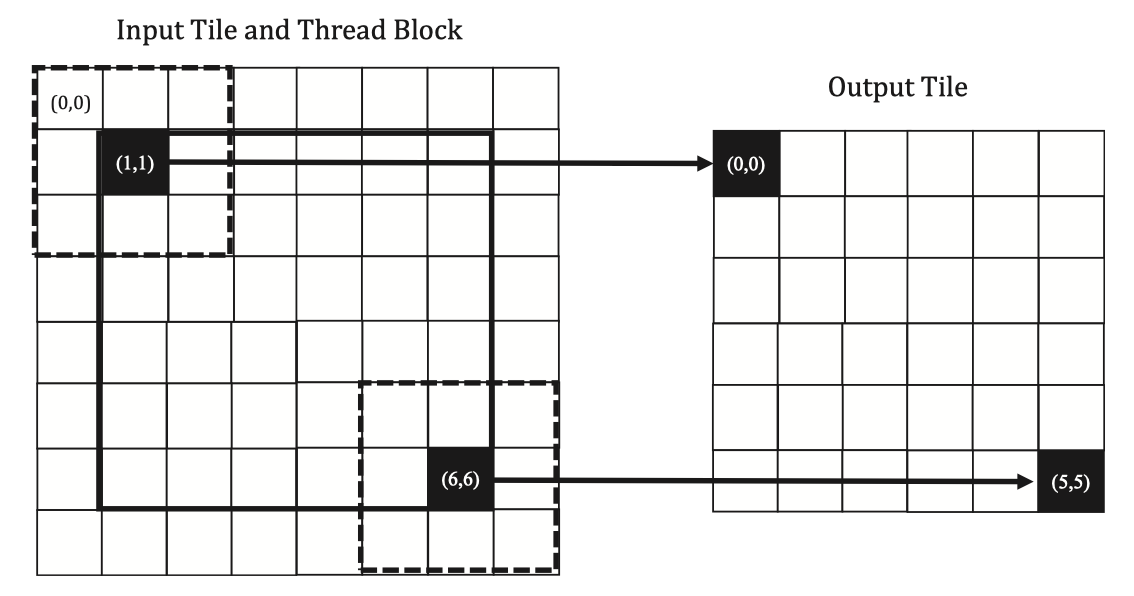
\includegraphics[width=0.9\textwidth]{figs/F7.13.png}
	\caption{\textit{一个小示例,说明使用共享内存中的输入图块元素来计算输出图块元素的线程组织。}}
\end{figure}

图 7.13 显示了使用 $3 \times 3$ 滤波器 (FILTER\_RADIUS=1)、$8 \times 8$ 个输入图块、
$8 \times 8$ 个块和 $6 \times 6$ 个输出图块进行卷积的小示例。 
图 7.13 的左侧显示了输入图块和线程块。 由于它们的大小相同,因此它们相互重叠。 
根据我们的设计,我们停用 FILTER\_RADIUS=1 外层线程。 
图 7.13 左侧中心的粗线框包围了用于计算输出图块元素的活动线程。 
在此示例中,活动线程的 threadIdx.x 和 threadIdx.y 值均在 1 到 6 的范围内。

图7.13还显示了活动线程到输出tile元素的映射:活动线程(tx,ty)将使用左上角为的输入tile元素的块来计算输出元素
(tx - FILTER\_RADIUS,ty - FILTER\_RADIUS) 输入图块的元素 (tx - FILTER\_RADIUS, ty - FILTER\_RADIUS)。 
这反映在图 7.12 的第 17-18 行中,其中列索引 (tileCol) 和行索引 (tileRow) 
分别分配为 threadIdx.x-FILTER\_RADIUS 和 threadId.y-FILTER\_RADIUS。

在图 7.13 的小例子中,线程 (1,1) 的tileCol 和tileRow 分别接收0 和0。 
因此,线程 (1, 1) 使用输入图块左上角的虚线框突出显示的 $3 \times 3$ 个输入图块元素块来计算输出图块的元素 (0,0)。 
fRow-fCol 循环嵌套在图 7.12 的第 24-28 行,迭代该块并生成输出元素。 
块中的线程(1,1)将迭代左上角为N\_s[0][0]的块,而线程(5,5)将迭代左上角为N\_s[5][5]的块。

在第 06-07 行中,blockIdx.x * OUT\_TILE\_DIM 和 blockIdx.y * OUT\_TILE\_DIM 
分别是分配给块的输出图块开头的水平和垂直 P 数组索引。 
正如我们之前讨论的,threadIdx.x-r 和 threadIdx.y-r 给出了图块的偏移量。 
因此 row 和 col 变量提供分配给每个活动线程的输出元素的索引。 每个线程使用这两个索引写入第 29 行中输出元素的最终值。

图 7.12 中的平铺 2D 卷积核比图 7.9 中的基本核更长、更复杂。 我们引入了额外的复杂性来减少 N 个元素的 DRAM 访问数量。 
目标是提高算术与全局内存访问的比率,以便所实现的性能不受 DRAM 带宽的限制或较少限制。 
回想一下 7.4 节,图 7.9 中内核的算术与全局内存访问比率是 0.5 OP/B。 现在让我们推导出图 7.12 中内核的这个比率。

对于处理数据边缘处的图块的块,处理幻影单元的线程不会对这些幻影单元执行任何存储器访问。 这减少了这些块的存储器访问次数。 
我们可以通过枚举使用每个幻影单元的线程数来计算减少的内存访问次数。 
然而,应该清楚的是,对于大型输入阵列,幻影单元对小掩模尺寸的影响将是微不足道的。 
因此,当我们计算平铺卷积核中的算术与全局内存访问比率时,我们将忽略幻影单元的影响,并仅考虑晕单元不是幻影单元的内部线程块。

我们现在计算图 7.12 中平铺内核的算术与全局内存访问比率。 
分配给输出图块元素的每个线程对过滤器的每个元素执行一次乘法和一次加法。 
因此,内部块中的线程共同执行 OUT\_TILE\_DIM$^2 *$ ($2*$ FILTER\_RADIUS + 1)$^2 *2$ 算术运算。 
至于全局内存访问,所有全局内存访问都已转移到将 N 个元素加载到共享内存的代码中。 
分配给输入图块元素的每个线程都会加载一个 4 字节输入值。 
因此 IN\_TILE\_DIM$^2 *4$=(OUT\_TILE\_DIM+$2*$ FILTER\_RADIUS)$^2 * 4$ 字节由每个内部块加载。 
因此,平铺内核的算术与全局内存访问比率为
\begin{equation*}
\frac{\text { OUT\_TILE\_DIM }^{2}*(2 * \text { FILTER\_RADIUS }+1)^{2}* 2}{(\text { OUT\_TILE\_DIM }+2 * \text { FILTER\_RADIUS })^{2} * 4}
\end{equation*}

对于我们具有 $5 \times 5$ 滤波器和 $32 \times 32$ 个输入图块($28 \times 28$ 个输出图块)的示例,
比率为 $\frac{28^{2} \times 5^{2} *2}{32^{2} * 4}=9.57 O P / B$。 
$32 \times 32$ 的输入图块大小是当前 GPU 可实现的最大大小。 
但是,我们可以对图块大小执行渐近分析,以获得此计算可实现的算术与全局内存访问比率的上限。 
如果 OUT\_TILE\_DIM 远大于 FILTER\_RADIUS,
我们可以认为 OUT\_TILE\_DIM+2 $\times$ FILTER\_RADIUS 约为 OUT\_TILE\_DIM。 
这将表达式简化为 (2 $\times$ FILTER\_RADIUS+1)$^2 * 2/4$。 这应该是一个非常直观的结果。 
在原始算法中,每个 N 个元素由大约 (2 $\times$ FILTER\_RADIUS+1) 2 个线程冗余加载,每个线程对其执行两次算术运算。 
因此,如果图块大小无限大,并且每个 4 字节元素仅加载到共享内存一次,
则比率应为 (2 $\times$ FILTER\_RADIUS+1)$^2 * 2/4$。

图 7.14 显示了不同滤波器大小的平铺卷积核的算术与全局内存访问比率如何随平铺尺寸变化,包括渐近界限。 
$5 \times 5$ 滤波器的比率范围为 12.5 OP/B。 然而,线程块大小限制为 $32 \times 32$ 时实际可实现的比率为 9.57 OP/B。 
对于较大的滤波器,例如图 7.14 底行中的 $9 \times 9$,比率的界限为 40.5 OP/B。 
然而,线程块大小限制为 $32 \times 32$ 时实际可实现的比率为 22.78 OP/B。 
因此,我们观察到过滤器尺寸越大,比率越高,因为每个输入元素被更多线程使用。 
然而,较大的滤波器尺寸在边界和实际实现的比率之间也具有较高的差异,因为较大数量的光环元素迫使输出图块较小。

\begin{figure}[H]
	\centering
	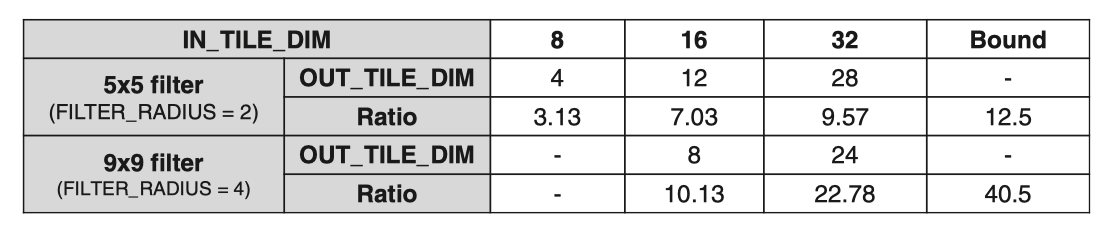
\includegraphics[width=0.9\textwidth]{figs/F7.14.png}
	\caption{\textit{算术与全局内存访问比作为 2D 平铺卷积的平铺大小和滤波器大小的函数。}}
\end{figure}

读者在使用小块和图块尺寸时应始终小心。 它们可能导致内存访问的减少明显少于预期。 
例如,在图 7.14 中,$7.8 \times 8$ 块(输入图块)仅导致 $5 \times 5$ 滤波器的 OP/B 比率为 3.13。 
在实践中,由于片上内存量不足,经常使用较小的瓦片尺寸,尤其是在 3D 卷积中,其中所需的片上存储器量随着瓦片的尺寸而快速增长。

\subsection{使用环状单元缓存的平铺卷积}
在图 7.12 中,代码的复杂性很大程度上与以下事实有关:由于光环单元的加载,输入图块和块比输出图块更大。 
回想一下,块的输入图块的光环单元也是相邻图块的内部元素。 
例如,在图 7.11 中,输入图块的浅阴影光环单元也是相邻块的输入图块的内部元素。 
当一个块需要其光环单元时,由于其相邻块的访问,它们很可能已经位于 L2 缓存中。 
因此,对这些光环单元的存储器访问可以自然地由 L2 高速缓存提供服务,而不会导致额外的 DRAM 流量。 
也就是说,我们可以将对这些光环单元的访问保留在原始N个元素中,而不是将它们加载到N\_ds中。 
我们现在提出一种平铺卷积算法,该算法对输入和输出平铺使用相同的维度,并且仅将每个平铺的内部元素加载到共享内存中。

\begin{figure}[H]
	\centering
	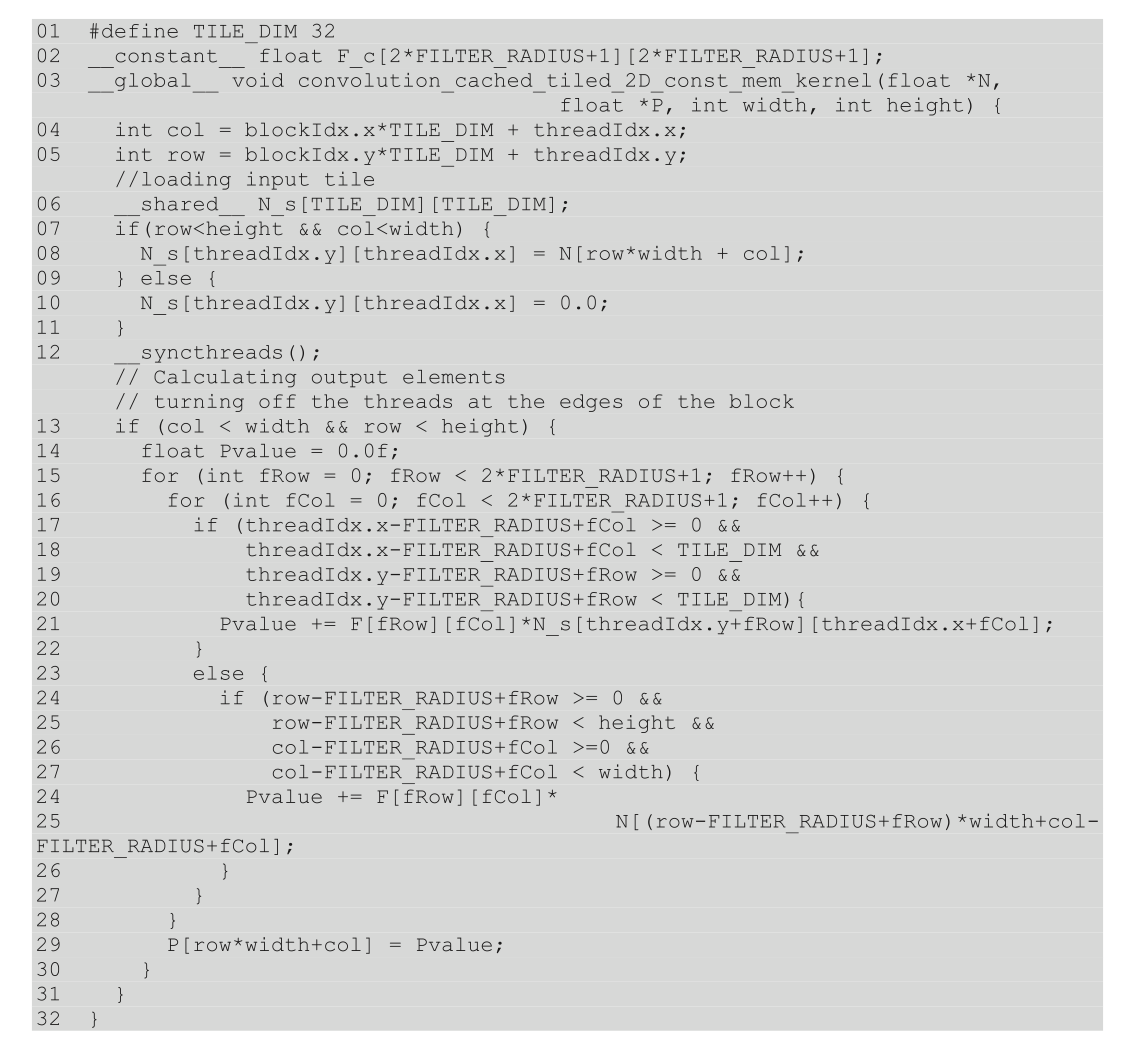
\includegraphics[width=0.9\textwidth]{figs/F7.15.png}
	\caption{\textit{使用光环缓存和 F 常量内存的平铺 2D 卷积核。}}
\end{figure}

图 7.15 显示了使用光环环单元缓存的 2D 卷积核。 在这个分片内核中,共享内存 N\_ds 数组只需保存分片的内部元素。 
因此,输入图块和输出图块具有相同的尺寸,其定义为常量 TILE\_DIM(第 1 行)。 
通过这种简化,N\_s 被声明为在 x 和 y 维度上都具有 TILE\_DIM 元素(第 6 行)。

因为输入图块和输出图块具有相同的尺寸,所以可以使用与输入/输出图块相同的尺寸来启动线程块。 
N\_s 元素的加载变得更简单,因为每个线程可以简单地加载与其指定的输出元素具有相同 x 和 y 坐标的输入元素(第 4-5 行和 7-11 行)。 
第 7 行还简化了加载输入元素的条件:因为内核不再将环状单元加载到共享内存中,所以不存在加载幻影单元的危险。 
因此,该条件仅需要检查图块可能超出输入数据的有效范围的通常边界条件。

然而,计算 P 元素的循环体变得更加复杂。 它需要添加条件来检查光环单元和幻影单元的使用。 
光环单元的处理是根据第 17-20 行中的条件完成的,该条件测试输入元素是否落入输入图块的内部。 
如果是,则从共享内存访问该元素。 如果不是,则第 24-27 行中的条件检查光环单元是否是幻影单元。 
如果是,则不会对该元素采取任何操作,因为我们假设幻影值为 0。否则,将从全局内存访问该元素。 
读者应验证处理幻影单元的条件是否与图 7.7 中使用的条件相似。

与图 7.12 中的内核相比,图 7.15 中的内核的一个微妙优点是,它的块大小、输入图块大小和输出图块大小可以相同,
并且可以是 2 的幂。因为输入图块大小和 图 7.12 中内核的输出块大小不同,在该内核执行期间可能存在更多内存分歧和控制分歧。

\subsection{总结}
在本章中,我们研究了卷积作为一种重要的并行计算模式。 虽然卷积被用于许多应用,例如计算机视觉和视频处理,
但它也代表了一种通用模式,构成了许多并行算法的基础。 例如,我们可以将偏微分方程求解器中的模板算法视为卷积的一种特殊情况; 
这将是第 8 章“模板”的主题。 再例如,也可以将网格点力或势值的计算视为卷积的一种特例,
这将在第17章“迭代磁共振成像重建”中介绍。 
我们还将在第 16 章“深度学习”中应用我们在本章中学到的有关卷积神经网络的大部分知识。

我们提出了一种基本的并行卷积算法,其实现将受到访问输入和滤波器元素的 DRAM 带宽的限制。 
然后,我们引入了常量内存并对内核和主机代码进行了简单修改,以利用常量缓存并消除对过滤器元素的几乎所有 DRAM 访问。 
我们进一步引入了平铺并行卷积算法,该算法通过利用共享内存来减少 DRAM 带宽消耗,同时引入更多的控制流发散和编程复杂性。 
最后,我们提出了一种平铺并行卷积算法,该算法利用 L1 和 L2 缓存来处理晕单元。

我们分析了平铺在提高算术与全局内存访问比率方面的优势。 分析是一项重要技能,有助于理解平铺对其他模式的好处。 
通过分析,我们可以了解小图块尺寸的限制,这对于大滤波器和 3D 卷积尤其明显。

尽管我们仅展示了 1D 和 2D 卷积的内核示例,但这些技术也直接适用于 3D 卷积。 
一般来说,由于维度较高,输入和输出数组的索引计算更加复杂。 
此外,每个线程都会有更多的循环嵌套,因为在加载图块和/或计算输出值时需要遍历多个维度。 
我们鼓励读者完成这些高维内核作为家庭作业。